% This file should be replaced with your file with thesis content.
%=========================================================================
% Authors: Michal Bidlo, Bohuslav Křena, Jaroslav Dytrych, Petr Veigend and Adam Herout 2019

% For compilation piecewise (see projekt.tex), it is necessary to uncomment it and change
% \documentclass[../projekt.tex]{subfiles}
% \begin{document}

\chapter{Introduction}
Over the last century, phones have changed from big and clumsy boxes that were mostly used to transfer simple spoken information over long distances into something different. Nowadays, mobile phones or smartphones are devices that allow us to navigate through big cities we have never been to before, translate conversations between people speaking different languages, find and recognize objects through the camera, and provide us with context.

Board games have likewise changed from the simplest ones, such as checkers, which can be played on any surface with a checkerboard pattern and rocks of different colors or shapes, into complex games that require players to study an entire book to play them correctly. An example of such a game would be Dungeons and Dragons and similar games. 

Having a device with a camera and hardware capable of analyzing images in our pockets could help solve problems with games that are too complex or just hard to learn. Applications that combine computer vision and board games ease the learning curve of games and shorten the time it takes for new players to grasp the basics of the game. These applications were called smart assistants by one of my predecessors who explored this topic. 

However, the main goal of this thesis is not to create a functional assistant application but rather to create an end-to-end computer vision pipeline that will help develop these applications.

Computer Vision Inference Library for Board Games, or CV.ILIBG, is an Android library written in Kotlin, whose purpose is to provide an abstract layer for developers that will allow them to speed up the development of applications that use computer vision to detect board game objects. Furthermore, the library contains template functions for loading assets, storing user data, and other useful tools for repetitive tasks.

Part of this pipeline is also a desktop application written in Python, whose purpose is to import unlabeled and unordered data; in this case, images, label them, create synthetic data that will enhance the results of the final model, and lastly, use a deep neural network trainer to turn them into models that can be used for object detection in the Android library.


\chapter{Literature}

\section{Computer Vision}
\subsection{Image Classification}
\subsection{Object detection}
\subsection{Kotlin coroutines}
\label{coroutines}
Concurrency in applications is a principle of performing multiple tasks at once. Traditionally this is done by creating a multiple threads and managing them, while this works it can became hard to maintain, for that reason Kotlin introduced coroutines \cite{kotlinCorountines}. Instead of manually managing all the parallel threads Kotlin allows developers to write parallel tasks in clean and sequential code.

\begin{figure}[hbt]
	\centering
	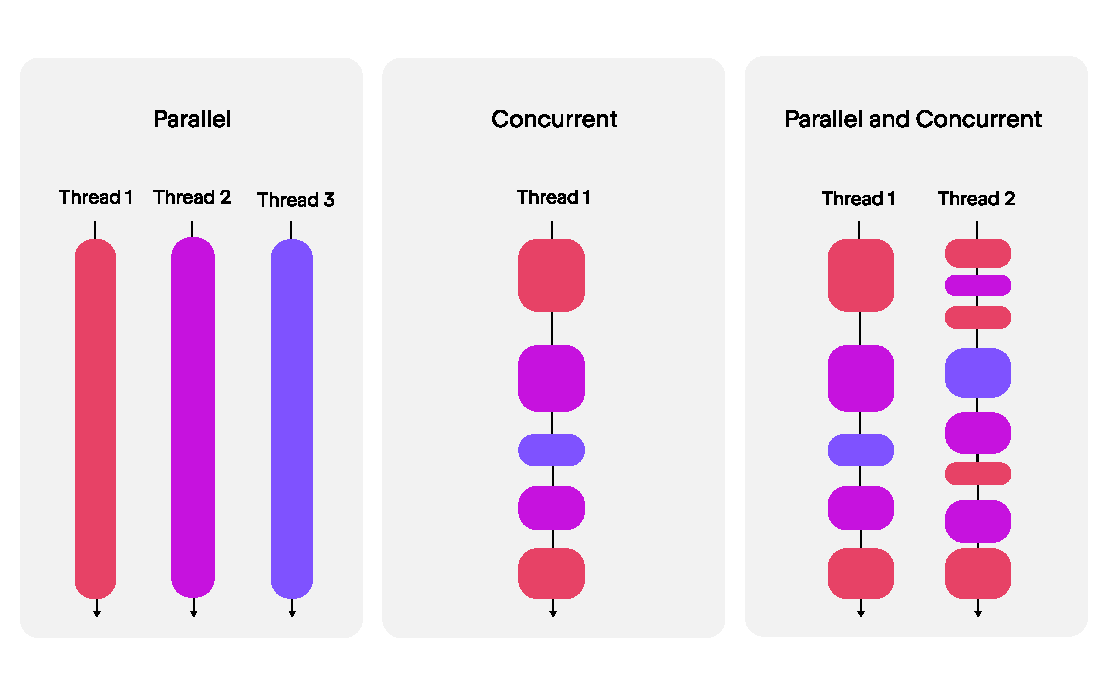
\includegraphics[width=0.7\textwidth]{obrazky-figures/parallelism-and-concurrency.pdf}
	\caption{Concurrency and parallelism. Source: \url{https://kotlinlang.org/docs/coroutines-basics.html}}
	\label{concurrencyimage}
\end{figure}

Suspended functions are functions that allow task or operations to be paused and later resumed. They are used for maintaining simple and clean sequential code that can run long operations, such as input/output operations, networking, or long calculations.

\textbf{TODO:}
\subsection{Other}


% ================================================================================================

% ================================================================================================

\section{Previous works}

% ================================================================================================

% ================================================================================================

\section{Card game Bang!}
Bang! is a western style card game for 4 to 7 players, with a suggested age of 8 or older. The game was created by Italian author Emiliano Sciarra \cite{bangWiki}, it was released in 2002 by the Italian publisher DV Giochi. In the Czech Republic and Slovak Republic, the game is released and manufactured by Albi. The game is very popular and has achieved 4 million sales worldwide.
\subsection{Rules of Bang!}

At the start of the game, players are randomly assigned one of the roles: Sheriff, Sheriffs assistant, Bandit, or Renegade. While the gameplay is the same for all the roles, their end goals are different. The role of the sheriff is to get rid of all the bandits and the renegade. The sheriff gets a bonus health, however, everybody knows who the sheriff is, while all other players must keep their role a secret. Assistants of sheriffs do not receive any bonuses, and their goal is the same as that of the sheriffs. Bandits, on the other hand, are targeting the sheriff and his assistants. The last role is a renegade, this role is trying to be the only player left in the game.

Except for the roles, players also get assigned characters. These modify how players play the game. For example, 
Lucky Duke allows the player to look at the top two cards and choose one of them instead of drawing at random.
Willy the Kid removes the limit on how many damaging cards Bang! can be played in one round.

The core principle of the game is simple: attack other players, defend and heal yourself, and lastly stop other players from achieving their goals while trying to achieve yours. The game can be relatively explosive, and players can be taken by surprise if other players group and start attacking them. The game itself doesn’t stop players from lying, deceiving, and forming groups to attack certain players, which makes it even trickier to play.

% ================================================================================================

% ================================================================================================

\chapter{Design of mobile library and desktop tool}
 
The goal of this project is to create an end-to-end computer vision pipeline that allows developers to build applications for mobile phones that utilize computer vision to detect game objects through the camera in their smartphones. The final applications should look something like this:

\begin{figure}[hbt]
	\centering
	\includegraphics[width=0.7\textwidth]{obrazky-figures/final_result_scheme.png}
	\caption{Image showing result application detecting Bang! cards.}
	\label{ResultApplicationScreenshot}
\end{figure}

The image above shows a mobile application detecting game objects, in this case, cards from the game Bang!. Detected cards are clickable and should bring the user to a detailed description. This should replace looking up rules in the games rule set and instead provide fast interfaces that will provide the user with information about game objects.


\section{Scheme of mobile library}

\begin{figure}[hbt]
	\centering
	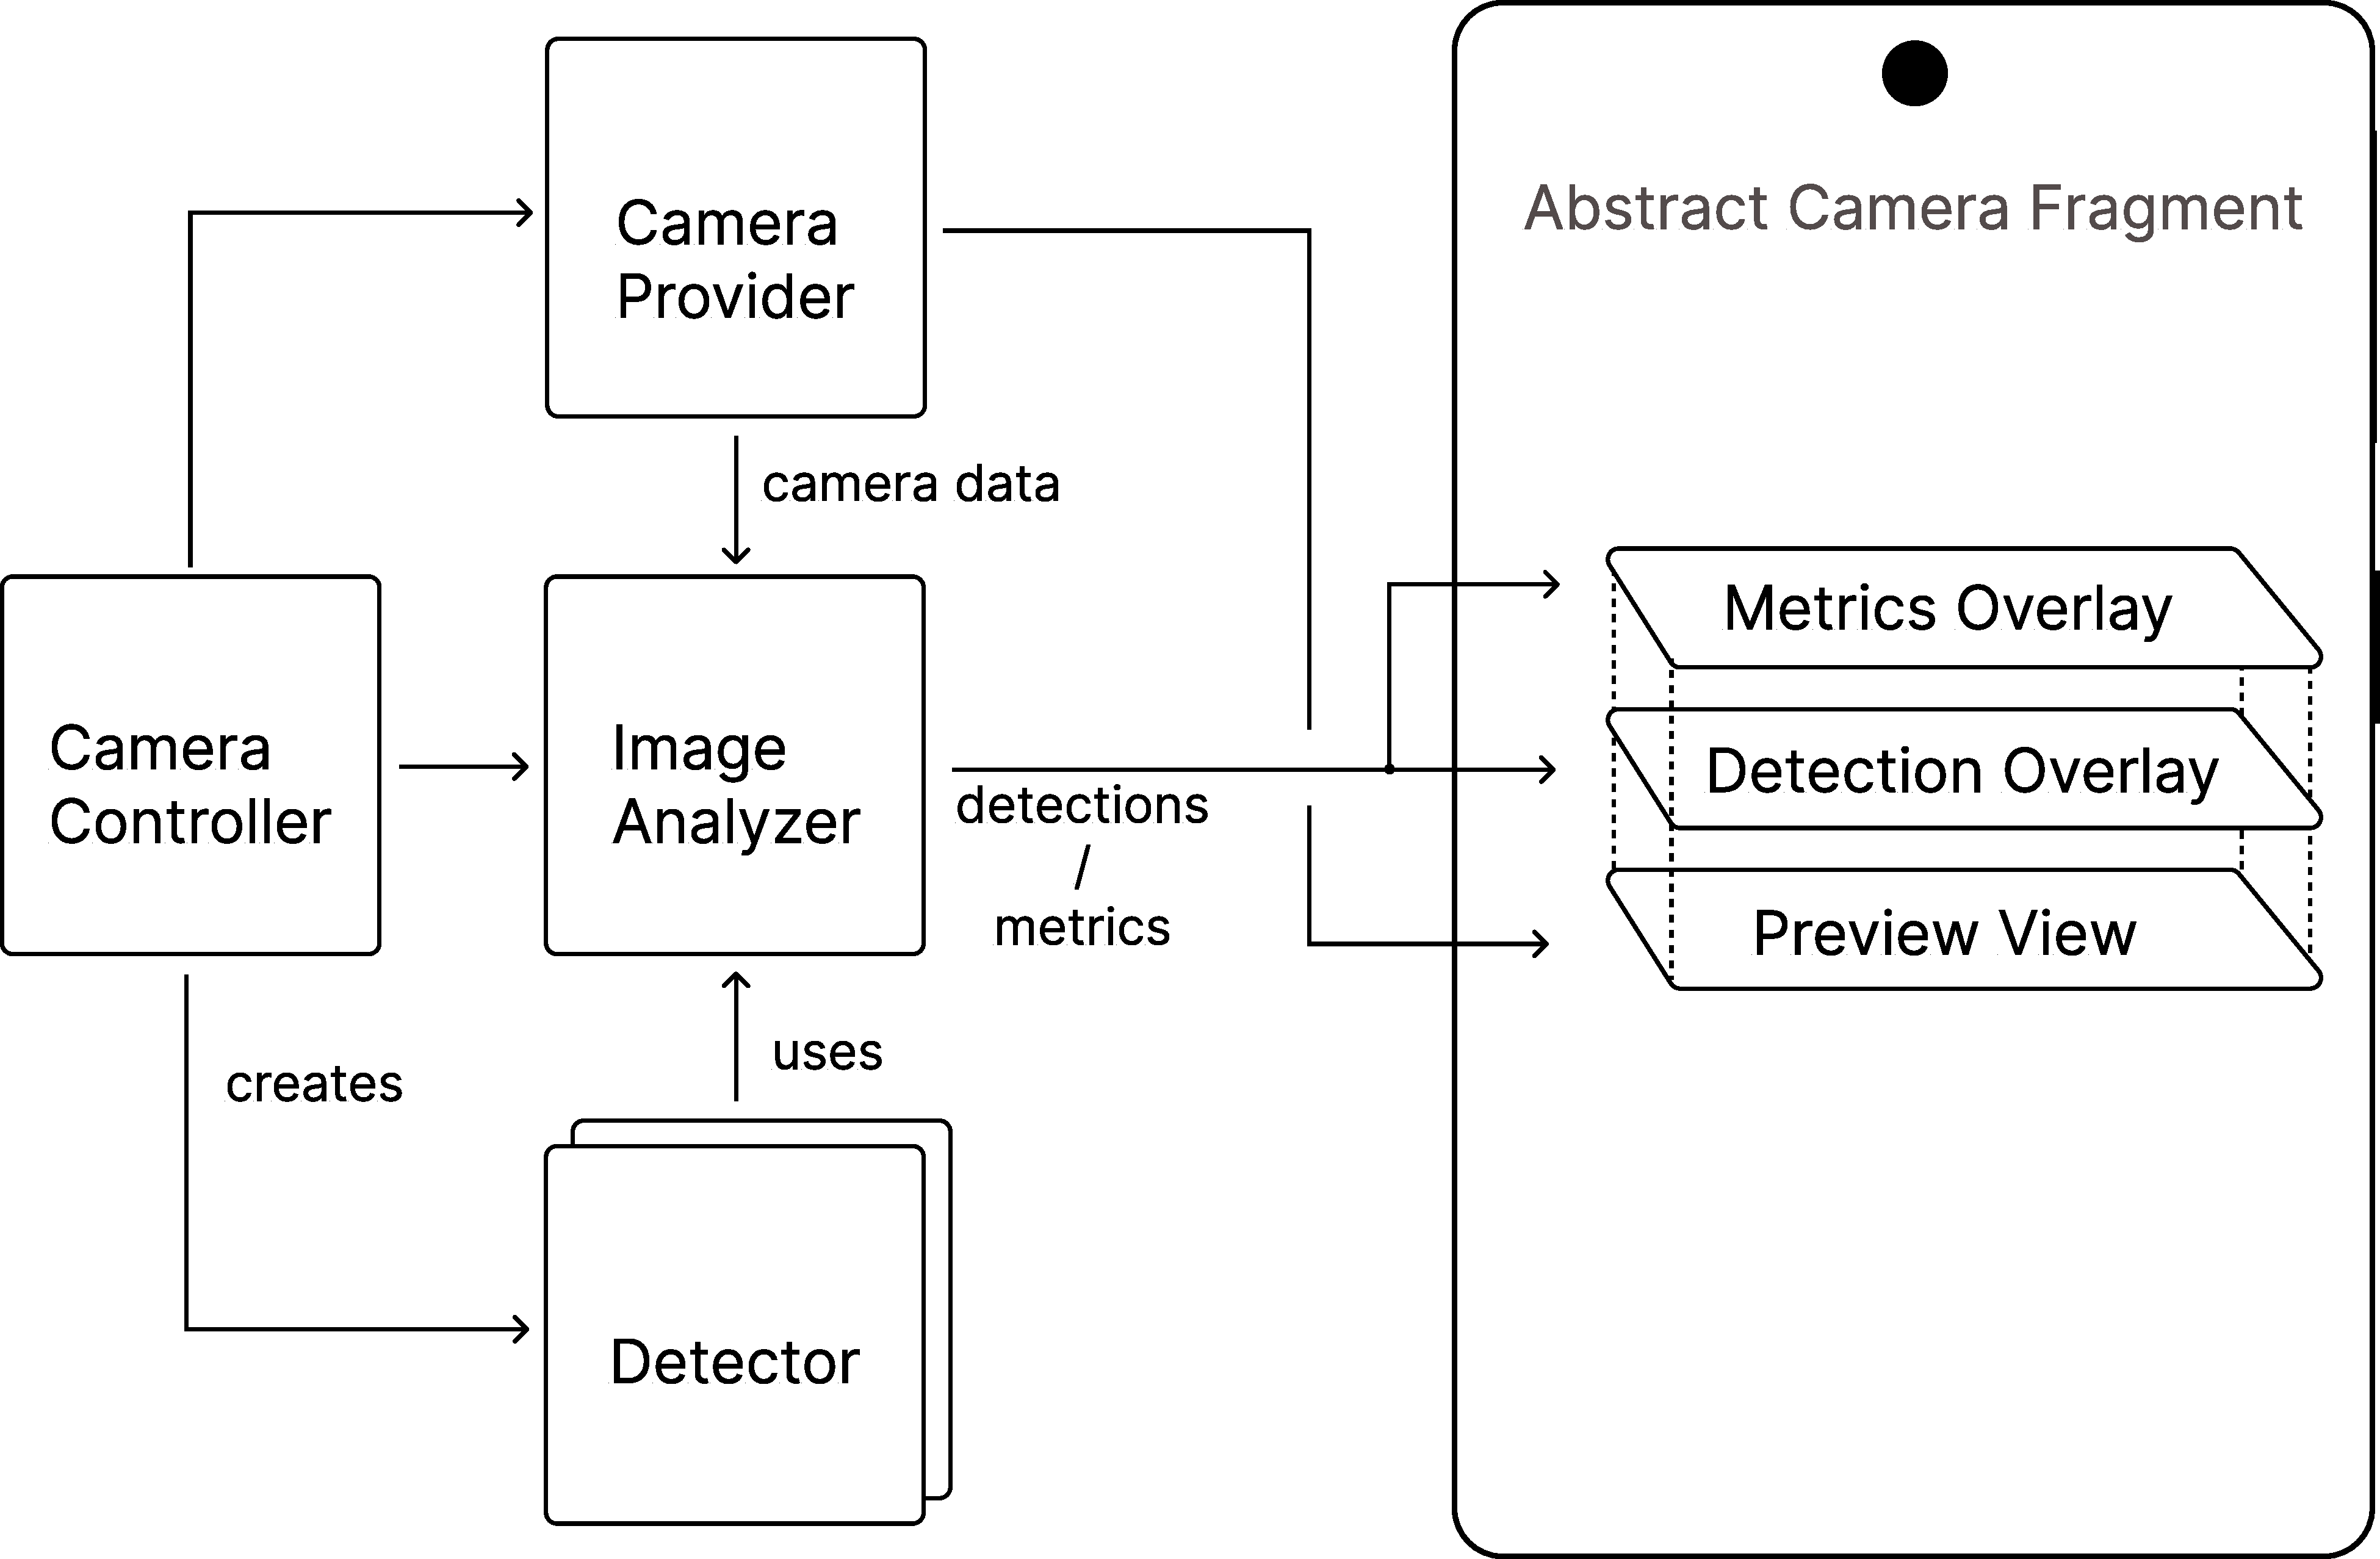
\includegraphics[width=0.7\textwidth]{obrazky-figures/mobile_library_abstract_scheme.pdf}
	\caption{Scheme of mobile library with high level of abstraction}
	\label{MobileLibraryScheem}
\end{figure}

This scheme shows the conceptual design of the proposed system.

The \textit{Camera Controller} is a core part of the system. Its purpose is to set up the camera.

Starting from the right, the \textit{Camera Controller} is a main part of this library, its purpose is to set up the \textit{Camera} and connect it to the \textit{Image Analyzer} that will analyze the output data from the camera. The \textit{camera controller} also provides \textit{Detectors} to the \textit{Image Analyzer}. The \textit{Image Analyzer} is a middleman that takes inputs from the \textit{Camera} , calls detection algorithms from the \textit{Detectors}, and lastly returns detected objects to the \textit{Overlay} , which will display these detections and also handle touch response. The last part is the \texttt{Camera Fragment}, which is responsible for handling UI elements and hosting the \texttt{Camera Controller}.

This architecture allows developers to use the existing \texttt{Camera Fragment} as a fully working base, while also allowing for simple extension of \texttt{Detectors}, \texttt{Detections Overlay}, or \texttt{Camera Fragment} to fully customize it for the needs of the game.
% ================================================================================================

% ================================================================================================


\chapter{Mobile library for board games}
This chapter starts with choosing a target mobile operating system, environment, and language for this library. Since the CV.ILIBG cannot work by itself, it needs a finished application that will imeplement parts of code such as navigation which are not part of the library and are left to developers to choose their own preferred solutions. However, in order to 


% ================================================================================================

% ================================================================================================

\section{Android development with Kotlin}
\subsection{Operating system}
Operating systems for mobile phones are mostly divided into two categories: those that use Android and those that use iOS. Since 2020, the smartphone market share has been steadily at 70\% \cite{phoneOsStatistics} in favor of Android over iOS. For this reason, the Android was chosen as the target operating system.


\subsection{Kotlin and Java}

For a long time, Java was the main programming language for Android development, however, that changed in 2019 \cite{androidKotlinBlog} when Google announced that it would be introducing the Kotlin language. As the blog claims, the Kotlin code is easier to understand, safer mainly for null exceptions, has exceptional concurrency handling, and mostly because it is interoperable with Java. The last point is the most crucial because it allows Kotlin code to use Java code and vise versa. This means that using Kotlin, which has less code overhead while keeping all the benefits and support of Java packages that were created over the long time of Java's existence. For this reason, Kotlin was chosen as the main programming language.


\subsection{Integrated Development Environment}
The most popular development environments (hereafter referred to as IDE) are Android Studio and IntelliJ Idea with Android development integrations. The developers of IntelliJ Idea posted a blog \cite{androidStudioAndIdea}
that explained the situation with Android Studio and IntelliJ Idea. The blog stated that Android Studio is based on IntelliJ Idea and uses the same internals. At first glance, both IDEs are similar, therefore, the choice was mostly a matter of personal preference, and I, as the author, leaned toward IntelliJ Idea due to a previous experience.


% ================================================================================================

% ================================================================================================

\section{OpenCV}
OpenCV \cite{opencv} is a multiplatform and multi-language open source library that provides algorithms for computer vision, machine learning, image manipulation, and many more. It is a well established library that is used by many companies and institutions, such as NASA. It supports Python, which is also used by desktop application for creating datasets and training models, but it also supports Java/Kotlin on mobile devices.  For this project, it was mostly used for image manipulation, both for creating synthetic data and for resizing and normalizing images from the camera to the correct format expected by the inference runtime that runs the object detection models.

% ================================================================================================

% ================================================================================================

\section{Choosing the inference engine}
To deploy a deep learning–based object detection model on embedded or mobile devices, a dedicated inference engine is required. Inference engines or runtimes are responsible for executing trained neural network models by loading the model parameters, processing input data, and producing task-specific outputs. In this work, the runtime executes a convolutional neural network–based object detection architecture to perform real-time object detection on image data.

OpenCV, with its \textit{Dnn} package, can be used as an inference engine, however, after the first trial deployment, the performance was not satisfactory for a real-time detector, and further research was needed. 

More popular and widely used are TensorFlow Lite and ONNX (Open Neural Network Exchange) Runtime. Both projects are backed by big companies such as Google and Microsoft, respectively, and both support mobile, sometimes also referred to as edge devices. A study from 2023 \cite{Ren2023_ONNX_TensorFlow_BScan} suggests that ONNX performs better on both CPU and GPU. The other blog post \cite{aimtechnoOnnxTFcomparison} from 2025 shows that the gap between the performance of the engines is smaller, and both have their pros and cons. The main difference is that ONNX Runtime is designed as an open standard and is better suited for multi-platform development, whereas TensorFlow Lite can benefit from Google's ecosystem.

Overall, the ONNX platform seems like a better choice as the core of the library, especially because of its open and multi-platform nature. However, since the library was made to be expandable, adding another inference engine is not out of the question.

% ================================================================================================

% ================================================================================================

\section{Implementation of Android application}
Until this point, the thesis contained mostly a theory, this section will describe the basic structure of an Android application and how the CV.ILIBG works with it. CV.ILIBG aims to simplify the development of Android applications that use computer vision, and this section should describe how it does exactly that. Most of the code and knowledge was gained from the official Android developer API website \cite{androiddev}.

% ================================================================================================

% ================================================================================================

\section{Application and activities}
\label{applicationClass}

The \texttt{Application()} class is the starting point of the life-cycle for all Android applications. In most projects, it is not necessary to use an \texttt{Application()} class, as it will be generated automatically. However, in order to use CV.ILIBG, it is necessary to create a subclass from the abstract \texttt{cv.CV.ILIBG.CustomApplication} and define \texttt{registerModels()} that links \texttt{Detector} classes to the correct model from the assets. More details are discussed in the subsection \ref{DetectorRegistry}.

% ================================================================================================

% ================================================================================================

\subsection{Activity classes and permissions to use camera}
Android API uses the \texttt{Activity}\footnote{Android Activity: \url{https://developer.android.com/reference/android/app/Activity}} class for creating a task specific parts of applications. Android usually uses \texttt{AppCompatActivity()} or \texttt{Fragments} \footnote{Android Fragments \url{https://developer.android.com/guide/fragments}} from the AndroidX \footnote{AndroidX is a refactored version of an Android API that is not bundled with the operating system: \url{https://developer.android.com/jetpack/androidx}}, for displaying content to users. 

CV.ILIBG does not interfere with this, nor does it provide any help with managing or navigating the activities. However, it is required for either the first activity that will be launched by the application or the activity that hosts the camera to request permissions to use it. 

That can be done by using \texttt{PermissionService} , which contains methods for that. This request should be placed in the overridden \texttt{onCreate()} method.

\begin{lstlisting}
    override fun onCreate(savedInstanceState: Bundle?) {
        super.onCreate(savedInstanceState)

        PermissionService.checkCameraPermission(this, this)
    }
\end{lstlisting}

These permissions also need to be added to the projects \texttt{AndroidManifest.xml} \footnote{Permissions for the AndroidManifest.xml: \url{https://developer.android.com/guide/topics/manifest/manifest-intro\#perms}} under the \texttt{manifest} element.

\begin{lstlisting}
    <?xml version="1.0" encoding="utf-8"?>
    <manifest xmlns:android = "http://schemas.android.com/apk/res/android">
        <uses-permission android:name = "android.permission.CAMERA"/>
    </manifest>
\end{lstlisting}

% ================================================================================================

% ================================================================================================

\section{AbstractCameraFragment()}
\label{AbstractCameraFragment}
\texttt{AbstractCameraFragment()} is a derived class from the Android Fragment that sets up 
\texttt{CameraController} (see \ref{CameraController}) and other user interface elements that are used by the controller. This class is abstract to prevent developers from using it as it is and to force them to derive from it should they choose to use it. 

\bigskip
\begin{lstlisting}
    class CameraFragment : AbstractCameraFragment(R.layout.fragment_camera) 
    {}
\end{lstlisting}
\bigskip

The code above shows \texttt{CameraFragment} class deriving from the \texttt{AbstractCameraFragment}. For the abstract class to work correctly, it is required that the \texttt{CameraFragment} contains these elements either by adding them in with Jetpack Compose toolkit \footnote{Jetpack compose: \url{https://developer.android.com/compose}} or by using XML-based view layouts. 
    
Both approaches are valid, and the choice depends on the developer’s preference, however, they must provide an elements that can be accessed by the \texttt{AbstractCameraFragment}. All of the listed elements with correct layout IDs and classes, or classes that are derived from them, must be found under the class derived from the \texttt{AbstractCameraFragment}.

\bigskip
\begin{minipage}{\textwidth}
\textbf{Format:} layout id: class or derived class

\begin{itemize}
  \item cameraxView: \texttt{androidx.camera.view.PreviewView}
  \item detectionOverlay: \texttt{DetectionOverlay}
  \item metricsOverlay: \texttt{MetricsOverlay}
  \item preciseDetectionButton: \texttt{ImageButton}
  \item exitPreciseDetectionButton: \texttt{ImageButton}
\end{itemize}
\end{minipage}
\bigskip

Should the developer decide to use different IDs, it is required to override the \texttt{initViews()} method with the correct \textit{R.id.ID} :
\bigskip
\begin{lstlisting}
protected open fun initViews(view: View) {
    cameraxView = view.findViewById<PreviewView>(R.id.ID)
    detectionOverlay = view.findViewById<DetectionOverlay>(R.id.ID)
    metricsOverlay = view.findViewById<MetricsOverlay>(R.id.ID)
    startQualityDetectionButton = view.findViewById<ImageButton>(R.id.ID)
    endQualityDetectionButton = view.findViewById<ImageButton>(R.id.ID)
}
\end{lstlisting}
\bigskip

\label{CameraFragmentOverlays}
In order for detections to be visible on top of the \texttt{previewView}, it is required that the camera fragment layout places the preview and overlays on top of each other with the same size.

\begin{figure}[hbt]
	\centering
	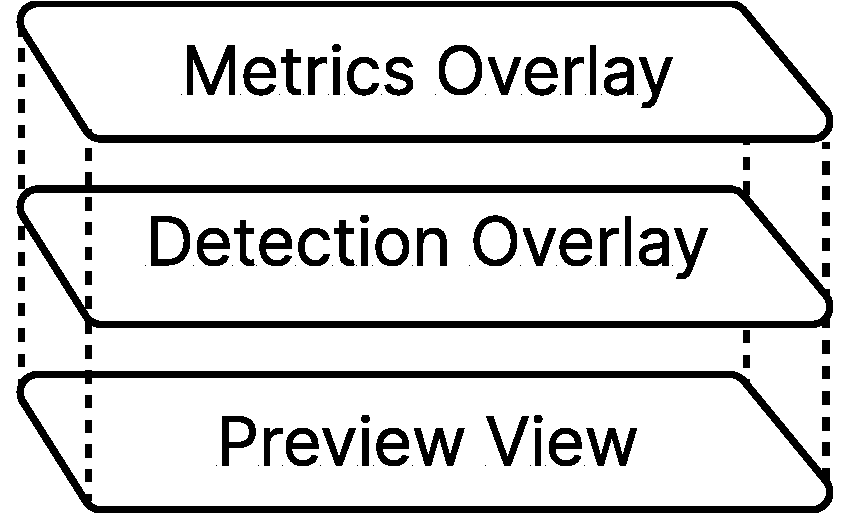
\includegraphics[width=0.4\textwidth]{obrazky-figures/camera_fragment_overlay.pdf}
	\caption{Scheme of mobile library with high level of abstraction}
	\label{MobileLibraryScheem}
\end{figure}


\subsection{Writing custom camera fragment}
This section describes how \texttt{AbstractCameraFragment} works for developers who do not want to use it and would rather implement it themselves.

First, override the \texttt{onViewCreated()} method and set the \texttt{PreviewView} \footnote{PreviewView: \url{https://developer.android.com/reference/androidx/camera/view/PreviewView}} scale type to \textit{FILL\_CENTER}. This will force the preview to keep the aspect ratio of the camera and scale camera images to fit the display, even if a small percentage of the image is lost. This is crucial as the \texttt{DetectionOverlay} will not scale detections properly without this option.

\bigskip
\begin{lstlisting}
    cameraxView.scaleType = PreviewView.ScaleType.FILL_CENTER
\end{lstlisting}
\bigskip

After setting the scale type, in the same overridden \texttt{onViewCreated()}, create an instance of the \texttt{CameraController} class and call its \texttt{start()} method to initialize it. The \texttt{start()} is a suspend function and needs to be called within the \texttt{lifecycle}. The \texttt{metricsOverlay} is optional. The \texttt{CameraController} constructor cannot fail or throw exceptions, however, the \texttt{start()} method can, and it is advised to use a try block for errors related to Android's \texttt{CameraProvider}\footnote{Camera Provider: \url{https://developer.android.com/reference/androidx/camera/core/CameraProvider?hl=en}}. Other errors and exceptions are handled by the \texttt{CameraController} \ref{CameraController}.

\bigskip
\begin{lstlisting}
    cameraController = CameraController(
        requireContext(),
        this as LifecycleOwner,
        cameraxView,
        detectionOverlay,
        metricsOverlay // nullable
    )

    lifecycleScope.launch {
        try {
            cameraController.start()
        } catch (e: Exception) {
            Log.e("CV", "Camera initialization failed: ${e.message}")
        }
    }
\end{lstlisting}
\bigskip

The last part of creating a custom camera fragment is to call the \texttt{destroy()} method of the \texttt{CameraController} once the fragment itself is going to destroyed. This can be achieved by simply overriding the \texttt{onDestroyView()} method.

\bigskip
\begin{lstlisting}
    override fun onDestroyView() {
        super.onDestroyView()
        cameraController.stop()
    }
\end{lstlisting}
\bigskip

% ================================================================================================

% ================================================================================================
 
\section{Camera Controller}
\label{CameraController}

The \texttt{CameraController} class is responsible for managing a \texttt{cameraProvider} that provides image data from the camera. It also manages \texttt{ImageAnalyzer} for analyzing image data and two \texttt{Detector} classes. The first \texttt{Detector} is a \texttt{realtimeDetector} that provides faster but less accurate detection for video-like object detection. The other \texttt{Detector} is a \texttt{quality} Detector that should provide more detailed detection models, which require more time and therefore would not be ideal for real-time object detection tasks. Switching between two modes is done with public methods \texttt{realtimeDetection()} and \texttt{qualityDetection()}. An actual logic for switching between two modes is implemented inside the \texttt{ImageAnalyzer}, see \ref{ImageAnalyzer}.

\subsection{Creating an instance}

\bigskip
\begin{lstlisting}
    class CameraController(
        private val context: Context,
        private val lifecycleOwner: LifecycleOwner,
        private val previewView: PreviewView,
        private val detectionOverlay: DetectionOverlay,
        private val metricsOverlay: MetricsOverlay?,    
        public val useRealtimeDetector: Boolean = true,
        public val useQualityDetector: Boolean = true )
\end{lstlisting}
\bigskip

An instance of \texttt{CameraController} requires:

\texttt{context} \footnote{Android Context: \url{https://developer.android.com/reference/android/content/Context}} of the activity that owns this current instance. The Context will be used for creating a \texttt{ProcessCameraProvider}, getting user preferences from the \texttt{SettingsService}, and lastly for showing the errors to the user using \texttt{AlertDialog} \footnote{Androids AlertDialog: \url{https://developer.android.com/reference/androidx/appcompat/app/AlertDialog?hl=en}}

\texttt{lifecycleOwner} \footnote{AndroidXs Lifecycle: \url{https://developer.android.com/topic/libraries/architecture/lifecycle}} is used for the \texttt{ProcessCameraProvider} to bind to a lifecycle. Internally, this allows the provider to react to changes in its owner, for example, stopping or resuming data capture.

\texttt{previewView} \footnote{PreviewView: \url{https://developer.android.com/reference/androidx/camera/view/PreviewView}} is a user interface element that displays data from the devices camera.

\texttt{detectionOverlay} is a view that will display detected objects and draw them on top of the \texttt{previewView}. As mentioned before, all layouts must be the same size, and on top of each other in the correct order, see \ref{CameraFragmentOverlays}. The \texttt{CameraController} does not use this overlay, instead, it uses it to create an instance of the \texttt{ImageAnalyzer}.

\texttt{metricsOverlay} is a simple overlay used for displaying the performance metrics of the \texttt{Detectors} onto the screen. This parameter is optional and targeted at developers as a debug tool. This overlay, like the \texttt{detectionOverlay}, is not used by the \texttt{CameraController} itself, instead, it is used to create an instance of the \texttt{ImageAnalyzer}.

\texttt{useRealtimeDetector} and \texttt{useQualityDetector} are boolean values used to decide whether the real-time or the quality detector should be created and used by the image analyzer. 

After creating an instance of the \texttt{CameraController}, it is required to initialize it with \texttt{start()} method, which is a \texttt{suspend function} and therefore can only be called from another suspend function or using a \texttt{Dispatcher}, \texttt{CoroutineScore.launch()} or \texttt{withContext()}, for more information on suspend functions, see \ref{coroutines} or \footnote{Coroutines and suspend function: \url{https://kotlinlang.org/docs/coroutines-basics.html\#create-your-first-coroutines}}


\subsection{CameraController.start()}
The \texttt{start()} method creates both \texttt{Detector} classes (see \ref{Detector}) and an instance of the \texttt{ImageAnalyzer} (see \ref{ImageAnalyzer}). The \texttt{ImageAnalyzer} is a class implementing the \texttt{ImageAnalysis.Analyzer} interface, which consists mainly of the \texttt{analyze()} method. This allows \texttt{cameraProvider} to send image data from the camera to the analyzer. However, the \texttt{cameraProvider} accepts only \texttt{androidx.camera.core.ImageAnalysis} that is built with a \texttt{.Builder()} method.

\bigskip
\begin{lstlisting}
    val imageAnalysis = ImageAnalysis.Builder()
        .setOutputImageRotationEnabled(true)
        .setResolutionSelector(resolutionSelector)
        .setBackpressureStrategy(ImageAnalysis.STRATEGY_KEEP_ONLY_LATEST)
        .build()
    imageAnalysis.setAnalyzer(cameraExecutor, imageAnalyzer!!)
\end{lstlisting}
\bigskip

Enabling image rotation will set \texttt{cameraProvider} to automatically rotate images for the \texttt{ImageAnalyzer} while introducing slight performance overhead. The backpressure strategy is set to \texttt{ImageAnalysis.STRATEGY\_KEEP\_ONLY\_LATEST} \cite{ImageAnalysisAndroid} and sets the behavior of the image analysis to store only the last image if the analysis of images is not keeping up with the production. Other strategies allow keeping the data in the queue; however, that is not desired, as it would block the preview, and the image would appear to be slow and tearing.

After creating an instance of \texttt{ImageAnalysis}, an \texttt{ImageAnalyzer} is set as its image analyzer alongside the \texttt{java.util.concurrent.ExecutorService}, which will execute \texttt{ImageAnalyzer} code on another thread. 

Since the \texttt{cameraExecutor} was created, it also needs to be destroyed with the \texttt{stop()} method to prevent memory leaks. The \texttt{stop()} method also destroys the \texttt{imageAnalyzer}, which allocates memory that needs to be manually released.

The last part of the \texttt{start()} method is setting the \texttt{previewView} as a \texttt{surfaceProvider} for the \texttt{preview} used by the \texttt{cameraProvider}. Lastly, binding the \texttt{imageAnalysis} and the \texttt{preview} to a lifecycle and the \texttt{cameraProvider}.

\subsection{start() - choosing resolution and the aspect ratio of the camera}

The \texttt{ImageAnalyzer} and the \texttt{CameraProvider} require a resolution at which they will operate. The resolution is set to the higher value between the \texttt{realtimeDetector.inputDataSize} and the \texttt{qualityDetector.inputDataSize}. If the camera cannot provide the resolution, it will use a
\begin{lstlisting}
    ResolutionStrategy.FALLBACK_RULE_CLOSEST_HIGHER_THEN_LOWER
\end{lstlisting}
which will choose the closest resolution that is higher than the specified one. 

Object detection models, such as YOLO, which is used in this project, usually expect a \texttt{640x640} screen resolution, which has a \texttt{1:1} aspect ratio. However, the displayed camera preview will be stretched across the whole display. Since the preview will crop the excess area to match the phone display, some data will be lost. Choosing an aspect ratio that is more similar to the display screen will minimize the loss of data and also reduce the number of detections that are outside of the displayed area. Therefore, the \texttt{16:9} aspect ratio was chosen as the default value. By comparing the statistics for mobile phone resolutions \cite{aspectRatioStats}, the most common ones are closer to \texttt{16:9} than to \texttt{4:3}.

\section{ImageAnalyzer}
\label{ImageAnalyzer}

The \texttt{ImageAnalyzer} class is an implementation of the \texttt{ImageAnalysis.Analyzer} interface. It 

\section{Setting up models with Detector Registry}
\label{DetectorRegistry}

\chapter{Demonstration application for the Bang!}
\label{bangApp}

\chapter{Dataset tool}


% ================================================================================================

% ================================================================================================

\section{Desktop GUI development with Python and Qt}
\subsection{Python}
\subsection{Qt/PySide6}


% ================================================================================================

% ================================================================================================

\section{Training deep neural networks for object detection}
\subsection{PyTorch}
\subsection{Ultralytics}


%=========================================================================

% For compilation piecewise (see projekt.tex), it is necessary to uncomment it
% \end{document}